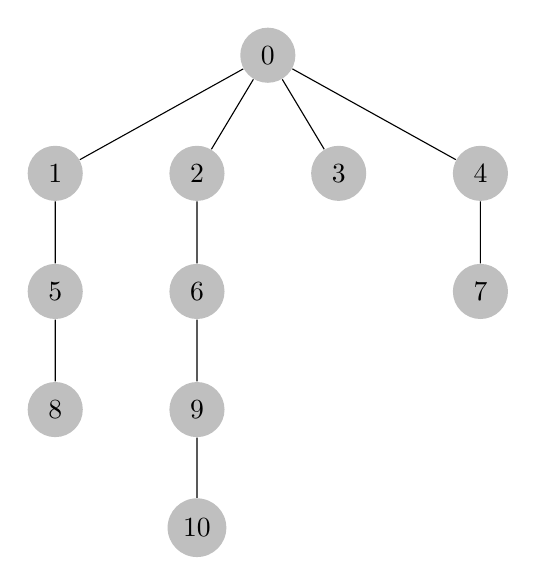
\begin{tikzpicture}[level/.style={sibling distance=18mm/#1}]
\tikzset{every node/.style={shape=circle,fill=black!25,minimum size=7mm}}
%\tikzset{every node/.style={shape=circle,
%                            font=\bfseries \Large,
%                            minimum size=3cm,
%                            scale=0.4
%                           }}
\node (root) {$0$}
    child {
        node {$1$}
        child {
            node (n5) {$5$}
            child {
                node {$8$}
            }
        }
    }
    child {node (n2) {$2$}
        child {node (n6) {$6$}
            child {node {$9$}
                child {node {$10$}
                }
            }
        }
    }
    child {node (n3) {$3$}
    }
    child {node (n4) {$4$}
        child {node {$7$}
        }
    }
    ;
\end{tikzpicture}
